\section{Blockchain suffix proofs}

We now provide a concrete non-interactive PoPoW construction which allows
proving certain predicates $Q$ of the chain $\chain$. The construction will
be done in two steps: First, we will build a construction which is limited to
a class of predicates that is easy to prove. Later, we will extend this class
of predicates by augmenting the construction.

Among the predicates which are stable, we now limit ourselves to the class of
predicates which are functions of only the chain suffix $\chain[-k:]$. We call
these predicates \textit{suffix sensitive}. As we will illustrate, these
predicates are significantly easier to prove, but at the same time seem to be
the most useful class of predicates which one needs for applications.

Specifically, these predicates allow proving that a recent transaction occurred
in the longest chain and in a block burried under $k$ blocks, which is
sufficient for verifying payments in the SPV case. Furthermore, these
predicates are expressive enough to describe the inclusion of the specific
recent transactions needed for building sidechains. Extending our construction,
we will generalize this class of predicates in a later section.

\subsection{Construction}

The \textsf{Verify} function of our NIPoPoW construction is described in
Algorithm~\ref{alg.nipopow-verifier}. The verifier algorithm is parameterized
by a predicate $Q$ and security parameters $k$ and $m$. The parameter $k$
pertains to the amount of proof-of-work needed to bury a block so that it is
believed to remain stable; in bitcoin's case, we often set $k = 6$. The
parameter $m$ is a security parameter pertaining to the prefix of the proof,
which connects the Genesis block to the $k$-sized suffix.  The verifier
receives several proofs by different provers in a collection of proofs
$\mathcal{P}$. Iterating over these proofs, it extracts the best one by
comparing these proofs. The comparison is done by calling the $\geq_m$
comparison algorithm. All proofs are checked for validity before comparison, in
particular that the first block of the suffix $\chi$ contains a pointer to the
last block of the prefix $\tilde\pi$. The exact structure of these parts of the
proofs will become clear momentarily when the prover algorithm is presented.

Note that the verifier evaluates the predicate $Q$ on a chain which has the
suffix $\chi$ and a fake prefix consisting of the empty block $\epsilon$
repeated as needed to form a chain of appropriate length. Because the predicate
only depends on the chain suffix, this does not make a difference. Observe as
well that the full chain $\chain$ is never sent to the verifier.

\import{./}{algorithms/alg.verifier-lite.tex}

The NIPoPoW proof construction is shown in Algorithm~\ref{alg.nipopow-prover}.
This produces a non-interactive PoPoW in parameter $m$ which consists of a
number of blocks for every level $\mu$. At the highest possible level at which
at least $m$ blocks, all these blocks are presented. Then, inductively, for
every superchain of level $\mu$ that is included in the proof, the suffix of
length $m$ is taken. Then the underlying superchain of level $\mu - 1$ covering
the same span as that suffix is also included, until level $0$ is reached. This
underlying superchain will have $2m$ blocks in expectation and always at least
$m$ blocks.

\import{./}{algorithms/alg.nipopow-prover.tex}

The algorithm returns a pair $(\tilde\pi, \chi)$. In this pair, $\chi$ is the
suffix of the blockchain containing the most recent $k$ blocks. $\tilde\pi$ is
a subchain of the underlying blockchain with the last $k$ blocks removed.
Because the blocks are combined into $\tilde\pi$ with the set union operator,
the proof will contain each block once, even if that block exists in multiple
superchain levels. When we take a $\mu$-superchain and are interested
in its last $m$ blocks, we fill the same range of blocks with blocks from the
superchain of level $\mu - 1$ below.  All the blocks of level $\mu$ which are
within this last $m$ blocks range will also be superblocks of level $\mu - 1$
and so we do not want to keep them in the proof structure twice.  Note
furthermore that no check is necessary to make sure the top-most level has at
least $m$ blocks, even though the verifier requires this. The reason is the
following: Assume the blockchain has at least $m$ blocks in total. Then when a
superchain of level $\mu$ has less than $m$ blocks in total, these blocks will
all be necessarily included into the proof by a lower-level superchain $\mu -
i$ for some $i > 0$.  Therefore, it does not hurt to add them to the set
$\tilde\pi$ earlier.

% \begin{figure}[h]
%     \caption{The first of a series of interactive proofs-of-proof-of-work for
%     $m = k = 3$. This proof is the only one that needs to be sent in case it
%     goes unchallenged.}
%     \centering
%     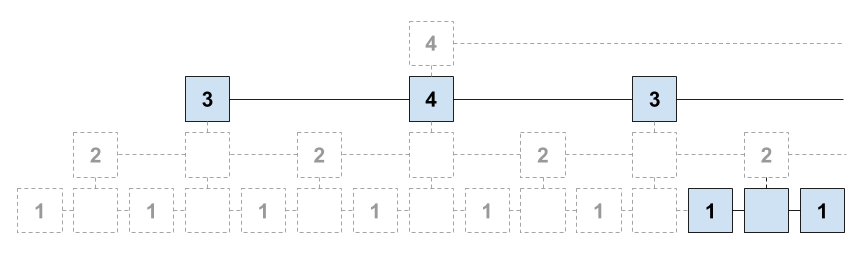
\includegraphics[width=0.5\textwidth,keepaspectratio]{figures/interactive-popow.png}
% \end{figure}

Figure~\ref{fig.nipopow} contains an example proof constructed for parameters
$m = k = 3$. The top superchain level which contains at least $m$ blocks is
level $\mu = 3$. For the $m$-sized suffix of that level, $5$ blocks of
superblock level $2$ are included for support spanning the same range. For the
last $3$ blocks of the level $2$ superchain, blocks of level $1$ are included
for support.

\begin{figure}[h]
    \caption{Non-interactive proof-of-work prefix for $m=k = 3$.}
    \centering
    \iftwocolumn
        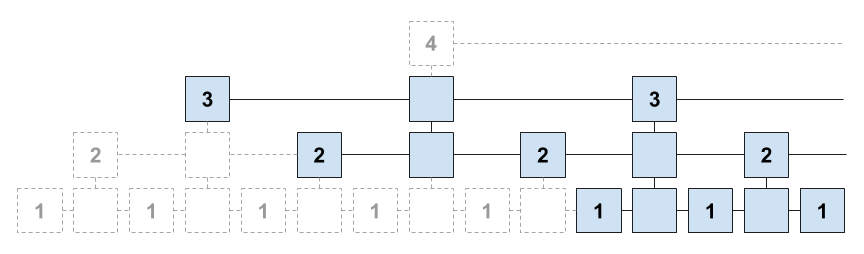
\includegraphics[width=\columnwidth,keepaspectratio]{figures/non-interactive-popow.png}
    \else
        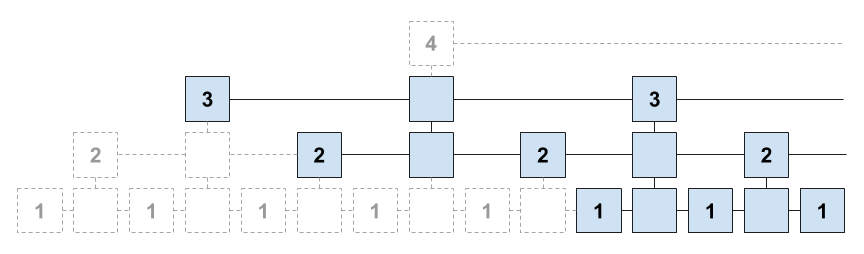
\includegraphics[width=0.7\columnwidth,keepaspectratio]{figures/non-interactive-popow.png}
    \fi
    \label{fig.nipopow}
\end{figure}

Finally, the $\geq_m$ operator which performs the actual comparison of proofs
is presented in Algorithm~\ref{alg.nipopow-maxchain}. It takes two proofs as
parameters and returns true if the first proof is winning, otherwise it return
false to indicate the second proof is winning. Initially the algorithm parses
the sets of blocks into chains by arranging them in topological order. It
rejects proofs that are not valid chains. It then computes the lowest common
ancestor block $b$ between the two proofs by calling the LCA function. Finally,
it finds the highest superblock level in which at least one of the proofs has
at least $m$ blocks. If the other one doesn't, then the one who does wins.
Otherwise, the one with most blocks wins. The number of blocks is counted using
the findInChain function, which returns the index of a block within the
respective superchain.

\import{./}{algorithms/alg.nipopow-maxchain.tex}
